\chapter{SVG feature representation}\label{chap:features}
Our goal is to extend beyond polyline modeling and capture the higher-level shapes of SVG objects.
Thus, one major challenge is to choose an adequate representation that captures all drawing information from an SVG and can be fed as an input vector to our neural network architecture.
Although many different elements are allowed by the SVG specification, including text, images, and basic shapes, we simplify the problem space to focus only on the generic \code{path} element since paths can be used to compose other elements. 

\section{Overview of SVG commands}
There are five commands possible in an SVG \code{path} as seen in Figure~\ref{fig:svg-commands}. Further detail about command parameters can be found in Table~\ref{tbl:svg-commands}~\cite{grasso2011svg}.

\begin{figure}[h]
    \centering
	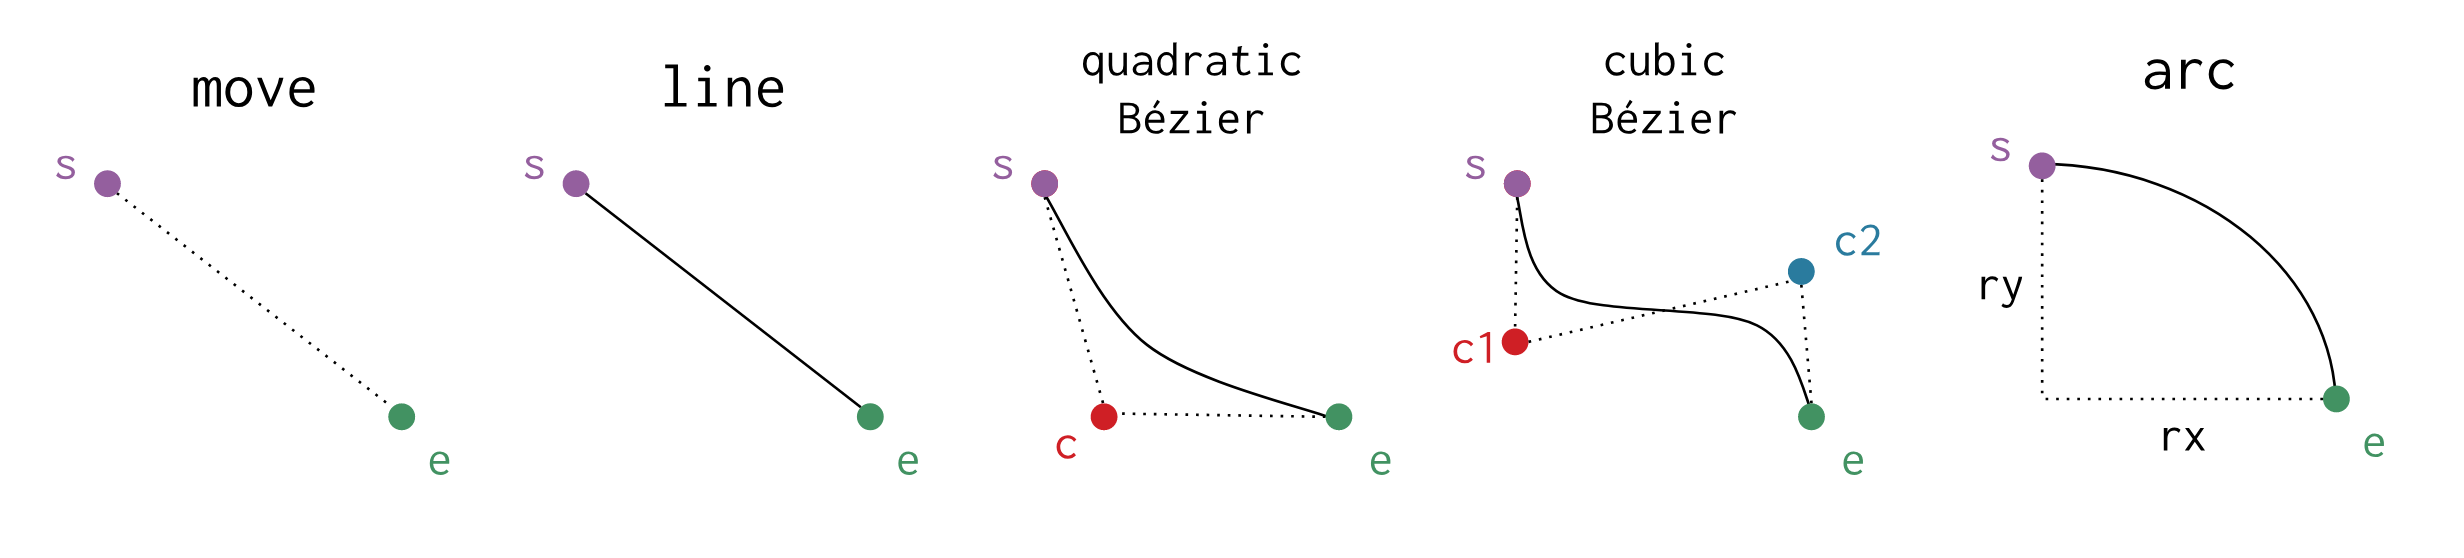
\includegraphics[width=\textwidth]{figures/commands}
    \caption{A visualization of the five commands in the SVG \code{path}\label{fig:svg-commands}}
\end{figure}


\begin{table}[h]
\centering
    \caption[The five possible commands in an SVG \code{path}]{A description of possible SVG path commands.
    For simplicity, we omit the relative coordinate variants of the commands, which specify $(dx, dy)$ coordinates instead of absolute $(x, y)$ for all control points.
    We also omit commands for vertical (\code{V}) and horizontal (\code{H}) lines as well as shorthand smoothed quadratic (\code{T}) and cubic (\code{S}) B\'eziers.\label{tbl:svg-commands}}
\begin{tabularx}{\linewidth}{l X}
\toprule
    Command & Code \& Description \\ \midrule
    Move & \code{M x y} \\
    & moves the pen to a specified point $(x, y)$ \\
    Line & \code{L x y} \\
    & draws a line from the current (start) point to the end point $(x, y)$ \\
    Quadratic B\'ezier & \code{Q cx cy, x y} \\
    & draws a quadratic B\'ezier curve according to given control point $(cx, cy)$ from the current point to the end point $(x, y)$ with the parametric equation $\textbf{B}(t) = (1-t)^2\textbf{s}+2(1-t)t\textbf{c} + t^2\textbf{e}$ \\
    Cubic B\'ezier & \code{C cx1 cy1, cx2 cy2, x y} \\
    & draws a cubic B\'ezier curve according to given control points $(cx_1, cy_1)$ and $(cx_2, cy_2)$ from the current point to the end point $(x, y)$ with the parametric equation $\textbf{B}(t) = (1-t)^3\textbf{s} + 3(1-t)^2t\textbf{c}_1 + 3(1-t)t^2\textbf{c}_2 + t^3\textbf{e}$\\
    Arc & \code{A rx ry t fl fs x y} \\
    & draws a section of an ellipse with the given $r_x$ and $r_y$ radii from the current point to the end point $(x, y)$ over angle $t$, with large-arc $f_l$ and sweep $f_s$ flags
\end{tabularx}
\end{table}

\section{Modeling SVGs}
We would like to model SVG inputs without loss of information about pen movements.
In essence, since SVGs name ordered lists of paths and their drawing commands, we model them as a sequence of mathematical parameters for the pen drawing commands and add a command for representing the transition between paths.
The sequential nature of this representation makes the generation task well-suited to a recurrent neural network architecture, as we cover in Chapter~\ref{chap:architecture}.

\subsection{Preprocessing}
SVG images often have additional properties like stroke and fill style.
As we focus on path generation exclusively, our first step in transforming input SVGs to a feature representation is to strip away those styles and focus only on the \code{path} elements of the input, often resulting in an image that depicts the outlines of the input shape---see Figure~\ref{fig:input_fonts} for examples.

Often, designers do not craft SVGs by editing XML by hand but rather with interactive image editing software such as Adobe Illustrator\footnote{\url{www.adobe.com/illustrator}} or Inkscape\footnote{\url{https://inkscape.org}}.
Thus, human-created SVGs often have varying path compositions, layers, and canvas sizes.

To constrain the modeling process, we first homogenize our dataset by preprocessing inputs, rescaling to the same overall canvas size (set to $256\times 256$ pixels) and reordering paths in the drawing sequence so that paths with larger bounding boxes are drawn first.

There is also variability in the directions and starting positions of path drawing.
Instead of controlling these factors in the preprocessing stage, our architecture is designed for bidirectionality, and all command sequences are interpreted such that the pen starts at coordinate $(0, 0)$ and moves to the first point in the input drawing.

\subsection{Simplifying path commands}
We aim to produce a system capable of modeling general SVGs, so inputs can contain any path command specified in Table~\ref{tbl:svg-commands}.
To avoid training bias and to constrain the problem space, we consolidate the different path commands into a single feature representation that encompasses all possible path pen movements.

Out of the five SVG path commands, three are parametric equations of differing degrees, so we can model these three (lines, quadratic B\'eziers, and cubic B\'eziers) using the parameter space for the highest degree cubic-order equation.
An elliptical arc segment, on the other hand, cannot be perfectly transformed into a cubic B\'ezier.
Arcs have five extra parameters used to describe them ($x$-radius, $y$-radius, angle of rotation, the large arc flag, and the sweep flag), so to compress their encoding we approximate them with the same parameter space as used for our parametric commands.
We use the method described in Appendix~\ref{app:algs} to approximate arc segments as cubic B\'eziers.

After all path drawing command types have been transformed to use the parameters needed for modeling cubic B\'ezier segments, we can represent each SVG command as a feature vector comprising those parameters and a three-dimensional one-hot pen state vector, similar to the feature representation used in~\cite{ha2017neural}.

Finally, for each \code{move} command and each disjoint path, we insert a feature vector that encodes the new end point and sets the pen state to note that the pen is up.

In all, our feature representation models each drawing command as a nine-dimensional vector (in contrast to the five-dimensional feature vector for polyline drawings in~\cite{ha2017neural}).
Six dimensions are used to model three $x, y$ coordinate parameters of cubic B\'eziers, and three dimensions are reserved for the \textit{pen down} ($p_d$), \textit{pen up} ($p_u$), and \textit{end drawing} ($p_e$) pen states.
Each input SVG is transformed into a sequence of commands, which is in turn translated into a sequence of these feature vectors.
In Chapter~\ref{chap:feature-variation}, we examine further details of this feature transformation process and how our representation modifications affect modeling performance.
